\documentclass[tikz,border=8pt]{standalone}
\usetikzlibrary{arrows.meta,decorations.pathmorphing,positioning}
\begin{document}
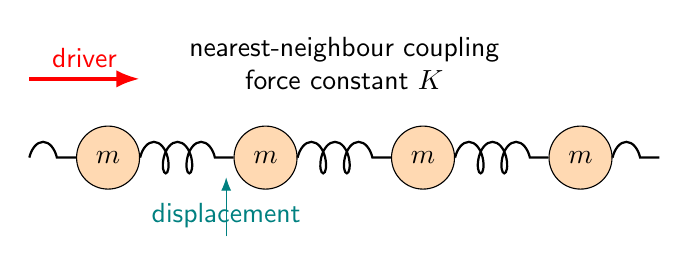
\begin{tikzpicture}[font=\sffamily,>=Latex,atom/.style={draw,circle,fill=orange!30,minimum size=8mm},spring/.style={decorate,decoration={coil,aspect=0.5,segment length=3mm,amplitude=2mm},thick}]
\node[atom] (a1) at (0,0) {$m$};
\node[atom] (a2) at (2,0) {$m$};
\node[atom] (a3) at (4,0) {$m$};
\node[atom] (a4) at (6,0) {$m$};
\draw[spring] (-1,0)--(a1.west);
\draw[spring] (a1.east)--(a2.west);
\draw[spring] (a2.east)--(a3.west);
\draw[spring] (a3.east)--(a4.west);
\draw[spring] (a4.east)--(7,0);
\draw[red,very thick,-Latex] (-1,1)--(.4,1) node[midway,above] {driver};
\draw[teal,->] (1.5,-1)--(1.5,-.25) node[below=2mm] {displacement};
\node[align=center] at (3,1.2) {nearest-neighbour coupling\\force constant $K$};
\end{tikzpicture}
\end{document}
